\setcounter{equation}{0}
\chapter{Revisão bibliográfica}
As concessionárias de energia elétrica e diversas instituições de pesquisa, nos últimos anos vêm trabalhando na busca de uma solução para a inspeção de linhas de transmissão de alta tensão. A abrangência de suas pesquisas perfazem em grande parte no desenvolvimento de robôs para realizar a inspeção. Este projeto de tese utilizará de um sistema mecânico desenvolvido no projeto do primeiro robô de inspeção de linha de transmissão brasileiro de baixo peso, apresentado no VII Congresso de Inovação Tecnológica em Energia Elétrica (ref). A escolha no uso desta solução mecânica deve-se aos resultados alcançados por este projeto diante dos desafios de uma inspeção de linhas de transmissão. Denominado projeto D311 e sob o código Aneel PD-4950-0311/2011, teve como objetivo
Apesar de alcançar os objetivos inicialmente traçados, o sistema de navegação do robô não era autônomo, seu deslocamento e transposição era baseado em reconhecimentos de padrões e todos os algoritmos pré-estabelecidos eram acionados quando do reconhecimento do padrão.
O presente projeto de tese propõe ser uma proposta inovadora em relação aos resultados alcançados descritos atualmente na literatura, atingindo uma navegação autônoma através do uso de técnicas de aprendizagem de máquinas.

\section{Projetos de relevância desenvolvidos}
Diante dos desafios e objetivos propostos neste projeto de tese, será exposto de forma sucinta alguns projetos e trabalhos desenvolvidos no âmbito dos robôs de inspeção de linha de transmissão.

Além dos projetos apresentados anteriormente, Pagnano et. al \cite{pag:13} se propõe a descrever um roadmap para o desenvolvimento futuro dos robôs de inspeção em linha de transmissão, reforçando o aspecto da autonomia dos robôs e sua confiabilidade na execução das transposições dos obstáculos.

\section{Navegação autônoma em robôs de inspeção de linhas de transmissão}
Localização e Mapeamento Simultâneos (SLAM) é um dos problemas fundamentais para a navegação autônoma de robôs [7], e por isso é um campo da robótica que vem sofrendo intensa pesquisa. Esse problema pode ser encarado como a dificuldade que um robô possui de, partindo de uma posição desconhecida, em um ambiente também desconhecido, construir um mapa dos locais já visitados e simultaneamente ser capaz de se localizar dentro desse mapa. Uma solução para esse problema permitiria o surgimento de robôs verdadeiramente autônomos, capazes de navegar de maneira segura por ambientes desconhecidos e cumprir objetivos sem a necessidade de auxílio externo de espécie alguma [8].
O mapeamento é um problema que consiste na integração de informações obtidas pelos sensores de um robô dentro de uma determinada representação. Este problema pode ser descrito pela pergunta "Com que o mundo se parece?”. Os aspectos centrais de mapeamento são a representação do ambiente e a interpretação dos dados do sensor. Em contraste com isso, a localização é o problema de estimar a posição do robô em relação a um mapa. Em outras palavras, o robô tem de responder à questão: “Onde eu estou?”. Normalmente, distingue-se entre uma posição de trajetória, onde a posição inicial do robô é conhecida, e localização global, em que não é dado nenhum conhecimento a priori sobre a posição de partida.
SLAM é definido como o problema de construção de um mapa e, ao mesmo tempo localizar o robô dentro desse mapa. Na prática, esses dois problemas não podem ser resolvidos de forma independente um do outro. Antes que um robô possa responder à questão com qual ambiente este se parece, a partir de um determinado conjunto de observações, ele precisa saber de que locais essas observações foram feitas. Ao mesmo tempo, é difícil estimar a posição atual de um robô sem um mapa. Portanto, SLAM é muitas vezes referido como o problema do ovo e da galinha: Um bom mapa é necessário para a localização, enquanto uma estimativa exata da posição é necessária para construir um mapa.


\section{Aprendizagem de máquinas}
O aspecto interativo do aprendizado de máquinas é importante porque, conforme os modelos são expostos a novos dados, eles são capazes de se adaptar de forma independente. Eles aprendem com os cálculos anteriores para produzir decisões e resultados confiáveis e reproduzíveis. O aprendizado de máquinas não é uma ciência nova, mas que está ganhando um novo impulso nestes últimos anos. Asmuth \cite{asm:13} aponta a importância de ressaltar que o conceito de aprendizado está relacionado com a melhoria do desempenho da rede segundo algum critério preestabelecido, no caso a abordagem bayesiana combinando informações anteriores com informações posteriores baseada nas observações obtidas por sensores. Os estudos de Asmuth \cite{asm:13} levaram a discussão de dois algoritmos de aprendizagem por reforço: BOSS (Best Of Sampled Set) e BFS3 (Bayesian Forward Search Sparse Sampling), fundamentados no modelo bayesiano. A figura \ref{asmuth} apresenta resumidamente a composição dos dois algoritmos.
%%%%%%%%%%%%%%%%%%%% PICTURE %%%%%%%%%%%%%%%%%%%%%%%%%%%%%%%
\begin{figure} [h!]												% Begin of the figure
	\centering													% Centering the figure
	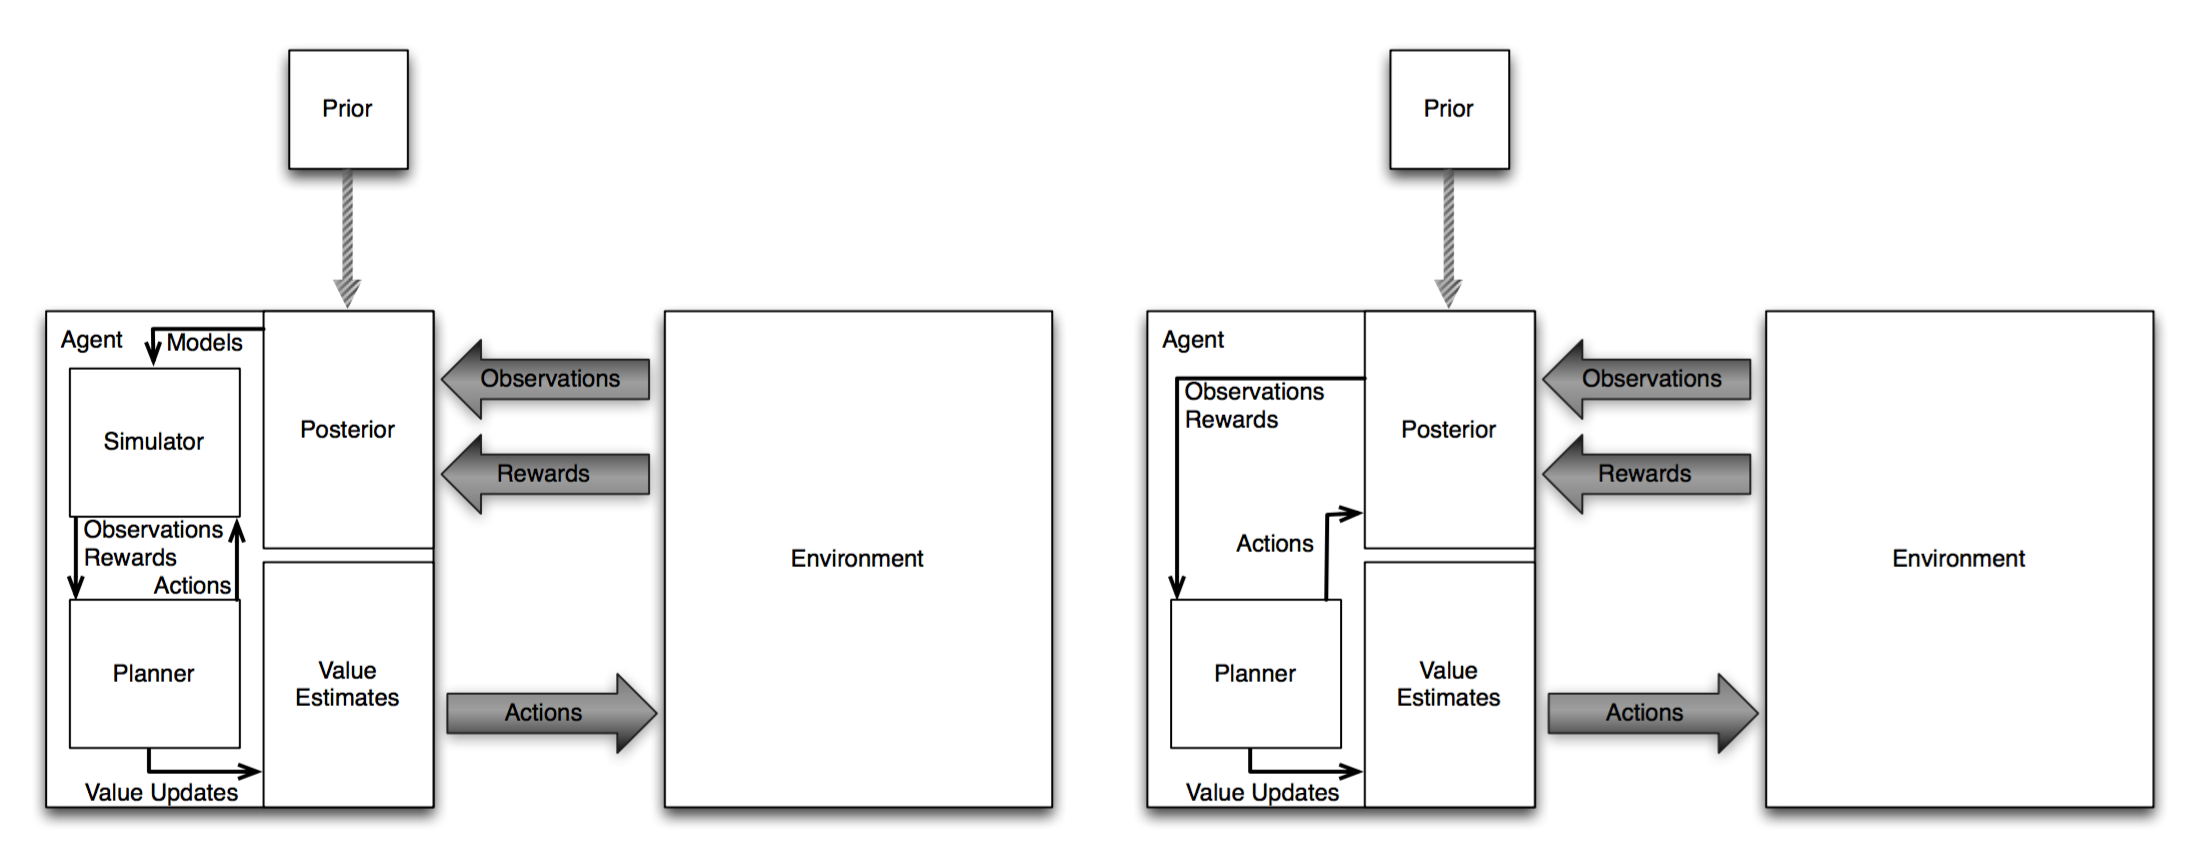
\includegraphics[width=1.0\textwidth]{./asmuth}				% Including picture
	\caption{Duas abordagens para o modelo Bayesiano baseado na aprendizagem de reforço, segundo Asmuth \cite{asm:13}.}			% Including title
	\label{asmuth}												% Caption of the figure
\end{figure}													% End of the figure
%%%%

Um outro modelo de reforço a ser investigado neste projeto de tese e que perfaz o tema central, é o Q-learning.

Q-learning é um algoritmo de aprendizado por reforço, atuando por diferença temporal. É um dos métodos mais simples de ser implementado. Sua regra de atualização é dada pela equação \ref{eq:qlearning}

\begin{equation} \label{eq:qlearning}
Q(s,a)=Q(s,a) + \alpha (r+\gamma  \underset{a'}{max} Q(s', a')-Q(s,a)) 	
\end{equation}

Dessa forma, quando o robô percorre o espaço de estados do ambiente e explora seu espaço de ações, uma tabela com os valores de $Q$ é construída. Dessa busca-se provar que os valores de $Q$ convergem para os valores $Q*$, caso o binômio (estado, ação) sejam visitados infinitas vezes. Com valores maiores, a probabilidade de se atingir máximos locais é maior. Benicasa \cite{ben:12} mostra  que o uso da técnica Q-learning mostra um retorno de convergência mais rápido quando comparado com outras técnicas, devido a sua maximização da recompensa média. Os testes realizados com a técnica Q-learning foram gerados através do algoritmo apresentado abaixo:\\

\hline\hline\\
\vspace*{0.2cm}
\noindent ALGORITMO Q-learning
\vspace*{0.2cm}
\hline\hline\\
\vspace*{0.5cm}
\noindent Inicie $Q(s,a)$ arbitrariamente;\\
{\bf for} cada episódio {\bf do}\\
\indent obtenha o estado atual $s$ do ambiente;\\
\indent {\bf for} cada passo do episódio {\bf do}\\
\indent \indent selecione uma ação $a$ \in {\bf A} $(s)$;\\

\indent \indent execute a ação $a$;\\
\indent \indent observe os valores de $s'$ e $r$;\\
\indent \indent atualize o valor de $Q(s,a)$;\\
\indent \indent $s$ \leftarrow $s'$;\\
\indent {\bf end}\\
{\bf end}\\
 
Segundo Benicasa \cite{ben:12}, com a implementação do algoritmo Q-learning a convergência do aprendizado Q-learning é muito mais rápida do que outras técnicas de aprendizagem.

O aprendizado supervisionado é baseado em um conjunto de exemplos de treinamento, em que as respostas desejadas são fornecidas. Com base neste conjunto, os algoritmos em geral generalizam para responder corretamente a todas as entradas possíveis. Marsland \cite{mar:09} denomina este tipo de aprendizado de utilização a partir de exemplos.

O aprendizado supervisionado se aplica a problemas em que se deseja obter um mapeamento entre padrões de entradas e saídas, a utilização neste projeto de tese será a aprendizagem on-line, onde o conjunto de dados muda continuamente, logo a rede deve estar em um contínuo processo de adaptação, buscando sempre uma otimização global.

Segundo Souza \cite{sou:14}, as técnicas bayesianas são abordagens eficientes em termos de avaliações da função que se pretende analisar, otimizando o conjunto de valores.
A otimização é um campo fundamental da matemática, mas para utilizá-la na aprendizagem de máquinas é preciso restringi-la \cite{bro:10}. Souza \cite{sou:14} define esta restrição pela maximização, logo a maximização de uma função de um valor real pode ser dada pela Equação \ref{eq:bayes1} e a maximização da função transformada $[-f(x)]$ é dada pela Equação \ref{eq:bayes2} .

\begin{equation} \label{eq:bayes1}
X^* = arg \underset{x}{max} f(x) 	
\end{equation}

ou mínimo

\begin{equation} \label{eq:bayes2}
X^* = arg \underset{x}{min} f(x)  = arg \underset{x}{max} (-f(x))
\end{equation}

Assim como apresentado na sucinta explanação sobre a aprendizagem por reforço, a aprendizagem supervisionada bayesiana também é modelada por um algoritmo. Brochu \cite{bro:10} modelou o algoritmo abaixo para encontra a função $f$ desconhecida, ou seja, para encontrar o máximo como definido na Equação \ref{eq:bayes1}.\\

\hline\hline\\
\vspace*{0.2cm}
\noindent ALGORITMO Bayesian
\vspace*{0.2cm}
\hline\hline\\
\vspace*{0.5cm}
\noindent ${\bf X_i}$ : ponto da amostra escolhido na interação $i$;\\
\noindent $s$ : função de aquisição;\\
\noindet $f$ : função desconhecida;\\
{\bf for} $i = 1,2,3 ...$ {\bf do}\\
\indent obtenha ${\bf X_i} = arg \underset{x}{max}$  $s({\bf X})$;\\
\indent adquira uma amostra de $f$ na posição ${\bf X_i}$;\\
\indent atualize o modelo de $f$ com a nova amostra;\\
{\bf end}\\


Em cada iteração uma nova posição da amostra é selecionada pelo conhecimento previamente adquirido. Ao maximizar a função de aquisição $s$, a melhor posição é selecionada para testar a função desconhecida.

%%%%%%%%%%%%%%%%%%%%%%%%%%%%%%%%%%%%%%%%%%%%%%%%%%%%%%%%%%%%
%%%%%%%%%%%%%%%%%%%%  NEW SECTION   %%%%%%%%%%%%%%%%%%%%%%%%
%%%%%%%%%%%%%%%%%%%%%%%%%%%%%%%%%%%%%%%%%%%%%%%%%%%%%%%%%%%%
\setcounter{equation}{0}
\section{Notations}
Let $S^h \subset H^1(\Omega)$ be finite element space defined by
\[S^h:=\{\chi \in C(\bar \Omega): \chi|_\tau \mbox{ is linear }
\forall \tau \in \mathcal{T}^h\} \subset H^1(\Omega).\]
Denote by $\{x_i\}_{i=1}^{J}$ the set of nodes of $ \mathcal{T}^h$
and let $ \{\eta_i\}_{i=1}^{J}$ be basis for $S^h$ defined by
$\eta_i(x_j)=\delta_{ij},$ for $i,j=1, \dots ,J$.

Let $\pi^h: C(\bar \Omega)\mapsto S^h $ be the interpolation
operator such that  $\pi^h\chi(x_i)=\chi(x_i),$ for $i=1, \dots , J$
and define a discrete inner product on $C(\bar \Omega)$ as follows
\begin{equation}
(\chi_1,\chi_2)^h:=\int_{\Omega}\pi^h(\chi_1(x)\chi_2(x))dx \equiv
\sum_{i=1}^{J}m_i\chi_1(x_i)\chi_2(x_i),\label{3S0000}
\end{equation}
where $m_i=(\eta_i,\eta_i)^h$. The induced norm
$\|\cdot\|_h:=[(\cdot,\cdot)^h]^{\frac{1}{2}}$ on $S^h$ is equivalent to
$|\cdot|_0:=[(\cdot,\cdot)]^{\frac{1}{2}}$.  Note that the integral
(\ref{3S0000}) can easily be computed by means of vertex quadrature
rule, which exact for piecewise linear functions.


%%%%%%%%%%%%%%%%%%%%%%%%%%%%%%%%%%%%%%%%%%%%%%%%%%%%%%%%%%%%
%%%%%%%%%%%%%%%%%%%%  NEW SECTION   %%%%%%%%%%%%%%%%%%%%%%%%
%%%%%%%%%%%%%%%%%%%%%%%%%%%%%%%%%%%%%%%%%%%%%%%%%%%%%%%%%%%%
\setcounter{equation}{0}
\section{Practical Algorithms}
\subsection{Iterative  Method for Scheme 1 \label{implicit}}
Let us expand $U_i$ and $W_i$, $i=1,2,$  in terms of the standard
nodal basis functions of the finite element space $S^h$, that
is,
\eqlabon 
\begin{align}
U^n_1=\sum_{i=1}^{J}U_{1,i}^n\eta_i,\quad W^n_1=\sum_{i=1}^{J}W_{1,i}^n\eta_i,\label{5E0001a}\\
U^n_2=\sum_{i=1}^{J}U_{2,i}^n\eta_i,\quad W^n_2=\sum_{i=1}^{J}W_{2,i}^n\eta_i,\label{5E0001b}
\end{align}
where $J$ be the number of node points. 
\eqlaboff

\subsubsection{Concluding Remarks}
To see a clear interaction between the solutions $U_1$ and $U_2$ in
terms of their physical meaning, it is worthwhile doing computational
experiment in three space dimensions


Given $N$, a positive integer, let $\Delta t= T/N$ denote a fixed time step,
and $t^k=k\Delta t$ where $k=0,\dots ,N.$  We focus
our attention on approximating ($\bv{\rm P}$) by the discrete scheme
defined as follows:\\
($\bv{\rm P}^{h,\Delta t}_1$) \quad Given $U_1^0, U_2^0$, find
$\{U_1^n, U_2^n, W_1^n, W_2^n\} \in S^h\times S^h\times S^h\times S^h,$ for  $n=1,\dots, N,$ such that
$\forall \eta \in S^h $
\eqlabon 
\begin{align} 
(\frac{U^n_{1}-U_1^{n-1}}{\Delta t} ,\eta)^h  = &- (\nabla W^n_{1} ,\nabla \eta  ),\label{4F0008}\\
(W^n_{1},\eta)^h  =(F_1(U_1^n,U_2^n), & \eta)^h+\gamma
(\nabla U^n_{1} ,\nabla \eta),\label{4F0009}\\
U^0_1=&\; P^h u_{1}^{0},\label{4F0010}\\
\intertext{and}
(\frac{U^n_{2}-U_2^{n-1}}{\Delta t},\eta)^h  = &- (\nabla W^n_{2} ,\nabla \eta ),\label{4F0011}\\
(W^n_{2},\eta)^h  =(F_2(U_1^n,U_2^n), & \eta)^h+\gamma(\nabla U^n_{2} ,\nabla \eta ),\label{4F0012}\\
U^0_2 = & \; P^h u_{2}^{0},\label{4F0013}
\end{align}
where
\begin{align}
F_1(U_1^n,U_2^n) & = ({U^n_1})^3- U^{n-1}_1  +
D(U^{n}_1+U^{n-1}_1+2)(U^{n-1}_2+1)^2,\label{4F0014}\\
F_2(U_1^n,U_2^n) & = ({U^n_2})^3- U^{n-1}_2 + 
D(U^{n}_2+U^{n-1}_2+2)(U^{n}_1+1)^2.\label{4F0015}
\end{align}
Note that (\ref{4F0008}--c) is independent of $U^n_2$ and
(\ref{4F0011}--f) is dependent on $U^n_1.$

%%%%%%%%%%%%%%%%%%%%%%%%%%%%%%%%%%%%%%%%%%%%%%%%%%%%%%%%%%%%
%%%%%%%%%%%%%%%%%%%%  NEW SECTION   %%%%%%%%%%%%%%%%%%%%%%%%
%%%%%%%%%%%%%%%%%%%%%%%%%%%%%%%%%%%%%%%%%%%%%%%%%%%%%%%%%%%%
\setcounter{equation}{0}
\section{Notation}
Let $\Omega$ be a bounded domain in $\mathbb{R}^d,\; d\leq3$ with
boundary $\partial\Omega$. For
$d=2,3$ we assume that $\partial\Omega$ is Lipschitz boundary. 
Through out this thesis we adopt the standard notation for
Sobolev spaces, denoting the norm of $W^{m,p}(\Omega)\, (m \in
{\mathbb N}, p \in [1,\infty])$ by $\|\cdot\|_{m,p}$ and semi-norm by
$|\cdot|_{m,p}.$   For $p=2$,  $W^{m,p}(\Omega)$ will be denoted by
$H^m$ with the associated norm and semi-norm written as 
$\|\cdot\|_{m}$ and $|\cdot|_{m}$, respectively. In addition we denote the
$L^2(\Omega)$ inner product over $\Omega$ by $(\cdot,\cdot)$ and
define the mean of integral
\[\mints \eta := \frac{1}{|\Omega|}(\eta,1)\quad \forall\eta \in L^1(\Omega).\]
We also use the following notation, for $1 \leq q < \infty,$
\begin{align*}
L^{q}(0,T;W^{m,p}(\Omega)):=& \; \left\{ \eta(x,t):\;  \eta(\cdot,t) \in W^{m,p}(\Omega), \int_0^T  \|\eta(\cdot,t)\|_{m,p}^q\; dt < \infty\right \},\\
L^{\infty}(0,T;W^{m,p}(\Omega)):=& \; \left\{ \eta(x,t):
\eta(\cdot,t) \in W^{m,p}(\Omega)
,\; \displaystyle{\operatornamewithlimits{ess\,sup}_{t\in (0,T)}} \|\eta(\cdot,t)\|_{m,p} < \infty\right \},
\end{align*}

For later purposes, we recall the \holder inequality for $u\in L^p,\; v\in L^q$
and $1<p<\infty,$
\begin{equation}
\int_\Omega |uv| dx \leq \bigg(\int_\Omega u^p dx\bigg)^{\frac{1}{p}}\bigg(
\int_\Omega v^q dx \bigg)^{\frac{1}{q}},\quad\mbox{where}\;\; \frac{1}{p}+\frac{1}{q}=1,\label{Holder}
\end{equation}
and the following well-known Sobolev
interpolation results: Let $p \in
[1,\infty],\, m \geq 1$ and $v \in W^{m,p}(\Omega)$.  Then
there are constants $C$ and $\mu=
\frac{d}{m}\left(\frac{1}{p}-\frac{1}{r}  \right )$ such that the
inequality
\begin{equation}
|v|_{0,r} \leq C|v|^{1-\mu}_{0,p} \|v\|^\mu_{m,p},\quad \mbox{ holds for
} 
r\in 
\begin{cases}
        \mbox{$[p,\infty]$}&  \mbox{ if }  m-\frac{d}{p} > 0,\\
        \mbox{$[p,\infty)$} &\mbox{ if } m-\frac{d}{p} = 0,\\
        \mbox{$[p,-\frac{d}{ m-d/p}]$}& \mbox{ if } m-\frac{d}{p} < 0.
\end{cases}\label{gagliar}
\end{equation}
We also state the following lemma, which will prove useful
in our subsequent analysis.

%=====another Lemma==================
\begin{Lem}\label{Lem201}
Let $u,v,\eta \in H^1{(\Omega)}$, $f=u-v$, $g=u^m v^{n-m}$, $m,n=0,1,2,$ and $n-m\geq
0$. Then for $d=1,2,3,$
\begin{align}
\bigg| \int_\Omega f g \eta dx \bigg| &\leq C |u-v|_0\; \|u\|_1^m\; \|v\|_1^{n-m}\; \|\eta\|_1.
\label{2le000}
\end{align}
\end{Lem}
\bproof
Note that using the Cauchy-Schwarz inequality we have
\begin{align*}
|(u)^m v^{n-m}|_{0,p}&\leq
\begin{cases}
|u|_{0,2mp}^m \;|v|_{0,2(n-m)p}^{(n-m)}&\mbox{for}\;\;
 n-m\neq 0,\;\;\mbox{and}\;\; m\neq 0,\\
|u|_{0,mp}^m \;\;\mbox{or}\;\;|v|_{0,(n-m)p}^{(n-m)}&\mbox{for}\;\;
 m= 0,\;\;\mbox{or}\;\; n-m= 0\;\;\mbox{respectively}.\\
\end{cases}
\end{align*}
Noting the  generalise H\"older inequality  and the result above we have
\begin{align*}
\bigg| \int_\Omega f g \eta dx \bigg| 
&\leq |u-v|_0\;|u^m v^{n-m}|_{0,3}\;|\eta|_{0,6},\\
&\leq |u-v|_0\;\;|\eta|_{0,6}
\begin{cases}
|u|_{0,6}^2\;&\mbox{for}\;\;m=2,\\
|u|_{0,6}\;|v|_{0,6} \;&\mbox{for}\;\;m=1,\\
|v|_{0,6}^2 \;&\mbox{for}\;\;m=0,\\
\end{cases}\\
&\leq C |u-v|_0\; \|u\|_1^m\; \|v\|_1^{n-m}\; \|\eta\|_1,
\end{align*}
where we have noted (\ref{gagliar}) to obtain the last inequality.
This ends the proof.\eproof

%%%%%%%%%%%%%%%%%%%%%%%%%%%%%%%%%%%%%%%%%%%%%%%%%%%%%%%%%%%%
%%%%%%%%%%%%%%%%%%%%  NEW SECTION   %%%%%%%%%%%%%%%%%%%%%%%%
%%%%%%%%%%%%%%%%%%%%%%%%%%%%%%%%%%%%%%%%%%%%%%%%%%%%%%%%%%%%
\setcounter{equation}{0}
\section{The Existence and Uniqueness of the Continuous Problem}
Given $\gamma > 0$ and $u_i^0\in H^1(\Omega)$, for $i=1,2,$ such that
$\|u_1^0\|_1+\|u_2^0\|_1\leq C$.  We consider the problem: \\
({\textbf P}) \quad Find
$\{u_i, w_i\}$  such that $u_i \in
H^1(0,T;(H^1(\Omega))')\cap L^\infty(0,T;H^1(\Omega))$ for $a.e.$\; $t\in(0,T)$, $ w_i \in L^2(0,T;H^1(\Omega))$ 
\eqlabon 
\begin{align} 
\left \langle\frac{\partial u_{1}}{\partial t},\eta \right\rangle
=\;& - (\nabla w_{1}  ,\nabla\eta ),\label{2B0000a}\\
(w_{1},\eta) =(\phi(u_1),\eta)+\;& \gamma (\nabla u_{1},\nabla\eta )+2D (\Psi_1(u_1,u_2),\eta),\label{2B0000b}\\
u_1(x,0) =\;&  u^0_1(x),\label{2B0000c}
\end{align}
and
\begin{align} 
\left\langle\frac{\partial u_{2}}{\partial t},\eta \right\rangle =\;&  - (\nabla w_{2}  ,\nabla\eta ),\label{2B0000d}\\
(w_{2},\eta) =(\phi(u_2),\eta)+\;& \gamma (\nabla u_{2},\nabla\eta )+2D(\Psi_2(u_1,u_2),\eta),\label{2B0000e}\\
u_2(x,0)=\;&  u^0_2(x),\label{2B0000f}
\end{align}
for all $\eta\in H^1(\Omega)$ for $a.e.$\; $t\in(0,T)$.
\eqlaboff

Let $\Omega$ be bounded domain in ${\mathbb R}^d (d\leq3)$ with
Lipschitz boundary $\partial\Omega.$  We consider a coupled pair of
Cahn-Hilliard Equations modelling a phase separation on a thin
film of binary liquid mixture coating substrate, which is wet by one
component denoted by A and the other by B:\\
Find $\{u_1(x,t),u_2(x,t)\}\in {\mathbb R}\times {\mathbb R}$ such
that
\eqlabon 
\begin{align} 
\frac{\partial u_{1}}{\partial t}&  = \Delta w_{1} \quad  \mbox{in}\;\;\Omega,t>0, \label{1a0001a}\\ 
\frac{\partial u_{2}}{\partial t}&  = \Delta w_{2} \quad \mbox{in}\;\;\Omega,t>0 ,\label{1a0001b}\\
\intertext{where}
w_{1}  &=  \frac{\delta F(u_{1},u_{2})}{\delta u_{1}}, \label{1a0001c}\\
w_{2}  &=  \frac{\delta F(u_{1},u_{2})}{\delta u_{2}},\label{1a0001d}\\ 
F(u_{1},u_{2})   &=   b_1u_1^4- a_1u_1^2+c_1|\nabla u_1|^2 \nonumber\\
   &\quad  + b_2u_2^4-  a_2u_2^2+c_2|\nabla u_2|^2 \nonumber\\
   &\quad  + D \left(u_1+ \sqrt{\frac{a_1}{2b_1}}\right )^2  \left(u_2+
       \sqrt{\frac{a_2}{2b_2}}\right)^2.\label{1a0001e}
\end{align}
Here ${\delta F}(u_{1},u_{2})/{\delta u_{i}}$, for $i=1,2,$ indicates the functional derivative.
The variable $u_1$ denotes a local concentration of A or B and $u_2$ indicates
the presence of a liquid or a vapour phase. $c_i$ denote the surface
tension of $u_i$.  The coefficient $a_i$ is proportional
to $T_{c_i}-T$, where $T_{c_1}$ corresponds to the critical
temperature of the A-B phase separation, and $T_{c_2}$ represents the critical
temperature of the
liquid-vapour phase separation.
\eqlaboff


If $a_1>0$, $ a_2 >0$, there
are two equilibrium phases for each field corresponding to $u_1 = \pm
\sqrt{\frac{a_1}{2b_1}}$ and $u_2 = \pm \sqrt{\frac{a_2}{2b_2}}$,
denote as $u_1^+$, $u_1^-$, $u_2^+$, and $u_2^-$.  The coupling $D$
energetically inhibits the existence of the phase denoted by the
$(u_1^+$, $u_2^+)$.  Thus we have three-phase system: liquid A
correspond to $(u_1^-$, $u_2^-)$ regions, liquid B to $(u_1^+$,
$u_2^-)$ regions and the vapour phase to $(u_1^-$, $u_2^+)$ regions.

If $D=0$, the problem reduces to two decoupled Cahn-Hilliard equations, which has
been discussed at length in the mathematical literature.  And for this type of problem, we do not have
liquid-vapour interfaces.

In Chapter 5 two practical algorithms (implicit an explicit methods)
for solving the finite element at each time step are suggested.    We
discuss the convergence theory for the implicit scheme, which used to
solve the system arising from Scheme~1.   We also discuss  in this
chapter some computational results for one and two space dimensions.
We only use the implicit scheme for all simulations. Before showing
some computational results, we discuss linear stability solutions in
one space dimension.


